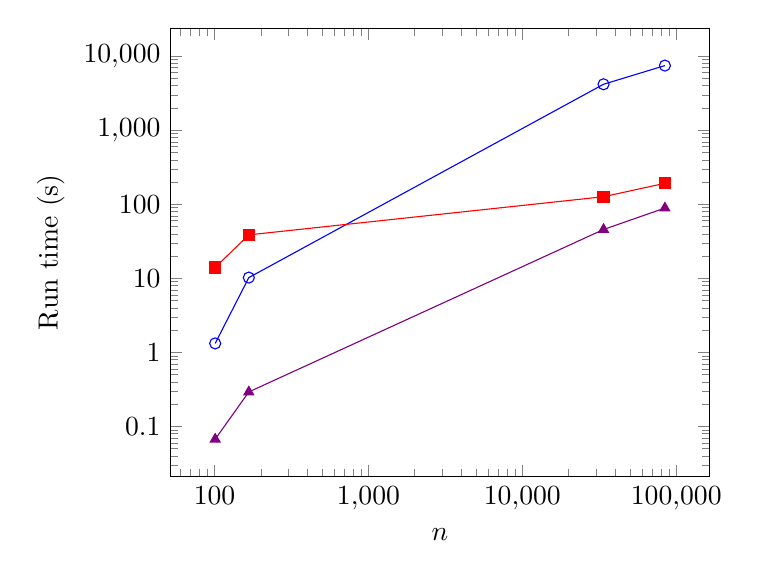
\begin{tikzpicture}
  \begin{loglogaxis}[xlabel=$n$,
			ylabel=Run time (s),
			log ticks with fixed point,
  ]
	%%
	%% Runtime for computing k number of graphs as a function of datasets' number of nodes
  %% Using Rods (stochastic graph generation)
	%%
  %	EMAIL CORE
  %	RADOSLAW
	%	enron (full)
	%	email-Enron.txt
  %% PHRG
  \addplot[color=blue, mark=o] table [col sep=comma]
			{
      101, 1.32355809212
      167, 10.2496099472
			33696, 4188.344877
      84384, 7487.98321414
      };
  %% CHLU
  \addplot[color=violet,mark=triangle*] table [col sep=comma]
    	{
      101, 0.0673129558563
      167, 0.292577981949
			33696, 45.7626059055
      84384, 89.1664869785
      };

  %% KRON
  \addplot[color=red,mark=square*] table [col sep=comma]
		  {
			101, 14.0635240078
      167, 38.7150030136
			33696, 126.776366949
      84384, 192.528311968
			};
    \end{loglogaxis}
\end{tikzpicture}
